\chapter{Results and Evaluation}

In this chapter, we assess the potential benefit of using SecureWilly in docker projects. Through experiments, we display the results of SecureWilly's execution and we evaluate the performance and the scalability of our software.

\section{Results}
\subsection{Benchmarks}
SecureWilly has been tested on creating AppArmor profiles for a set of multi-service projects provided by CloudSuite, a benchmark suite for cloud services. \cite{cloudsuite}

\subsubsection{Media-Streaming}
\textbf{Description}

One of the benchmarks of Cloudsuite that was used in the experimental evaluation was media-streaming. 

This benchmark uses the Nginx web server as a streaming server for hosted videos of various lengths and qualities. The client, based on httperf's wsesslog session generator, generates a request mix for different videos, to stress the server. \cite{mediastr}

The benchmark has two tiers: the server and the clients. The server runs Nginx, and the clients send requests to stream videos from the server. Each tier has its own image which is identified by its tag.

The streaming server requires a video dataset to serve and a synthetic dataset is generated, comprising several videos of different lengths and qualities. A separate docker image that handles the dataset generation is provided, which is then used to launch a dataset container that exposes a volume containing the video dataset.
\hfill\break

\textbf{Analysis of the profiles produced}

In the particular example, the benchmark was executed, having one client. SecureWilly produced one profile for each of the three services of the benchmark.
 
\underline{Rules}

In Figure 5.1, a line graph illustrates the amount of rules of each service's profile over the test plan runs.

All of the services start with non-zero amount of rules, which derives from static analysis's preliminary profiles.

We observe that most of the services had a gradual increase in their AppArmor profiles' rules, except for dataset, which starts with a preliminary profile of three rules and remains stable for the rest of the runs. This behaviour of dataset's profile is expected as the corresponding container does not execute any operations, but it only exists in order to expose a volume.

Server's and client's profiles follow a similar escalation, as they both rise to a point and then stabilize over the last runs. The rising derives from the first complain runs, in which rules are extracted gradually, as the addition of some rules leads to new system logs. While the first runs are crucial as the most part of the rules are extracted, the logs finally become gradually fewer until all actions are allowed, and this explains the final stability of the profiles, shown in the graph.

It appears that there is a threshold in runs, which represents the minimum number of runs which have to be executed, until a profile stabilizes over runs.

\begin{figure}[h!]
  \centering
   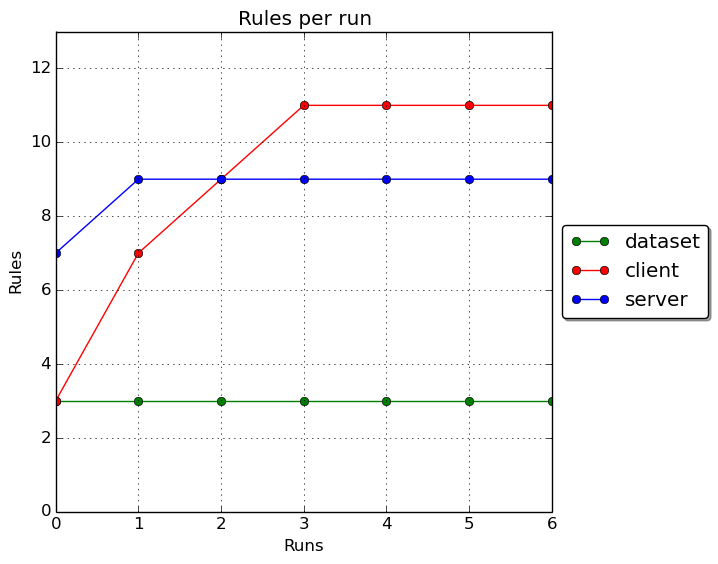
\includegraphics[width=0.85\linewidth]{./figures/mediastreaming/plots_with_grid/rules.png}
   \caption{Media Streaming: Rules per run for each service}
\end{figure}

The next step of the rules' analysis, was to identify which types of rules are encountered in our profiles. Figures 5.2, 5.3 and 5.4 shows a bar graph of the types of different rules used in the final AppArmor profile of each service. 

\begin{textblock*}{18cm}(0.1cm,5.6cm) % {block width} (coords)
\begin{figure}
  \begin{minipage}[H!]{0.55\textwidth}
    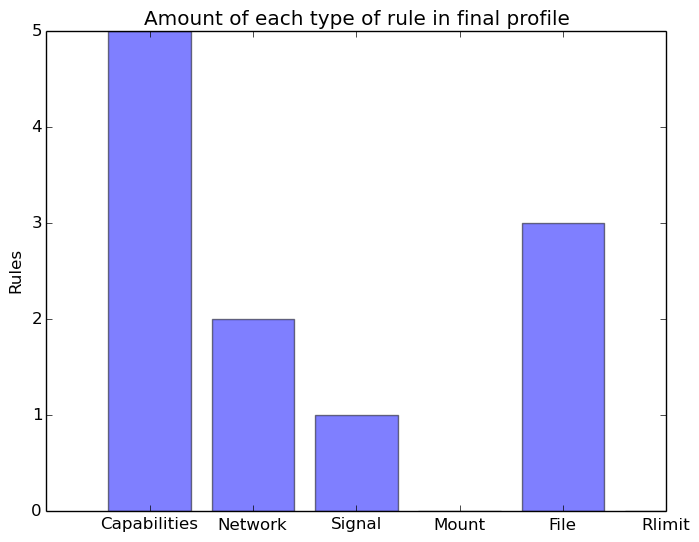
\includegraphics[width=\textwidth]{./figures/mediastreaming/plots_with_grid/Barfinal_cloudsuitemedia-streamingserver.png}
    \caption{Server's types of rules}
  \end{minipage}
  \begin{minipage}[H!]{0.55\textwidth}
    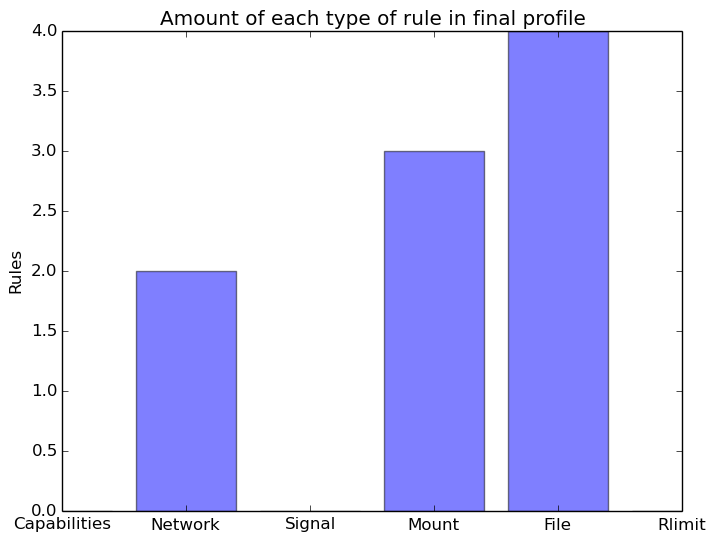
\includegraphics[width=\textwidth]{./figures/mediastreaming/plots_with_grid/Barfinal_cloudsuitemedia-streamingclient.png}
    \caption{Client's types of rules}
  \end{minipage}
\end{figure}
\end{textblock*}

\hfill\break\hfill\break\hfill\break\hfill\break\hfill\break\hfill\break\hfill\break\hfill\break\hfill\break\hfill\break\hfill\break\hfill\break\hfill\break\hfill\break\hfill\break\hfill\break\hfill\break

\begin{figure}[h!]
  \centering
   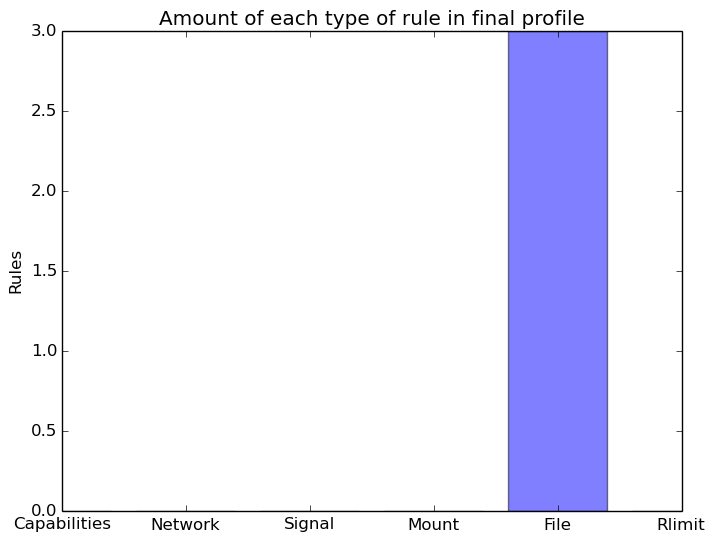
\includegraphics[width=0.64\linewidth]{./figures/mediastreaming/plots_with_grid/Barfinal_cloudsuitemedia-streamingdataset.png}
   \caption{Dataset's types of rules}
\end{figure}

The above bar graphs show that each profile describes perfectly the role of the service and the operations of its task.

In server's profile, the graph shows that a server has more capabilities rules than other types. This derives from the fact that a server commits several actions in order to serve the clients, and thus it is expected to need some capabilities. The file rules can derive from file access the server needs, but not from volumes since there are no mount rules extracted. Network rules are extracted for the internal communication of the services and lastly, one signal rule, which is needed in order to send a SEGKILL/SIGTERM to the server, since it is running as a daemon.

In client's profile, it appears that client had bind volumes, since there are mount rules and the corresponding file rules. File rules are more, because the preliminary profile's rules are added to them. Moreover, client also needs some network rules in order to communicate with the server.

As it is expeted, dataset only needs some file rules which are the ones of the preliminary profile, as its container will not commit any actions.

In the light of the above, it is clear that the AppArmor profile that are produced by SecureWilly are adjusted completely to the docker project and are closely tied with their tasks. That means they are efficient and secure, since they allow to the docker project to run unhinderedly, but all redundant actions will be denied.
\\
Let's see how the rules of each type increment over the runs of the test plan.

\begin{figure}[h!]
  \centering
   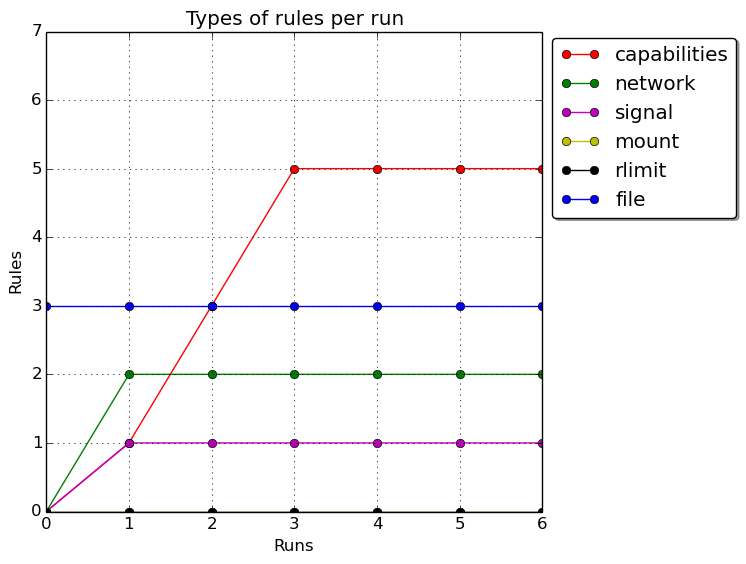
\includegraphics[width=0.64\linewidth]{./figures/mediastreaming/plots_with_grid/types_cloudsuitemedia-streamingserver.png}
   \caption{Server's types of rules per run}
\end{figure}

\begin{figure}[h!]
  \centering
   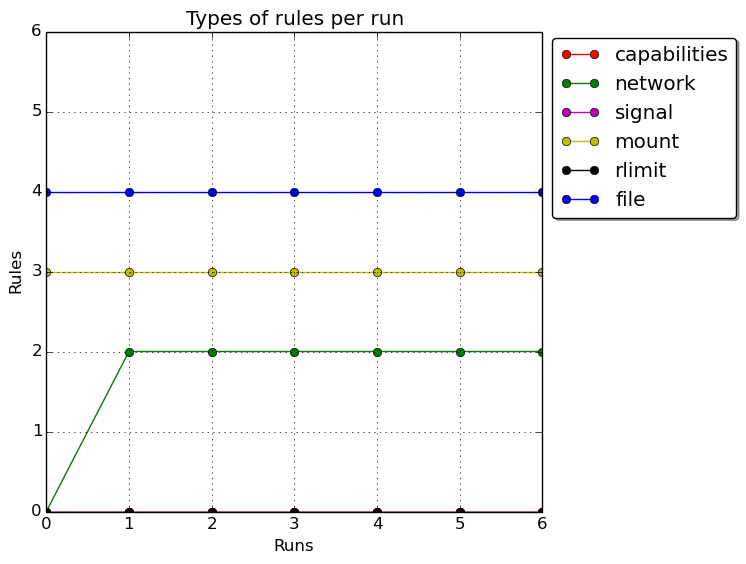
\includegraphics[width=0.64\linewidth]{./figures/mediastreaming/plots_with_grid/types_cloudsuitemedia-streamingclient.png}
   \caption{Client's types of rules per run}
\end{figure}

\begin{figure}[h!]
  \centering
   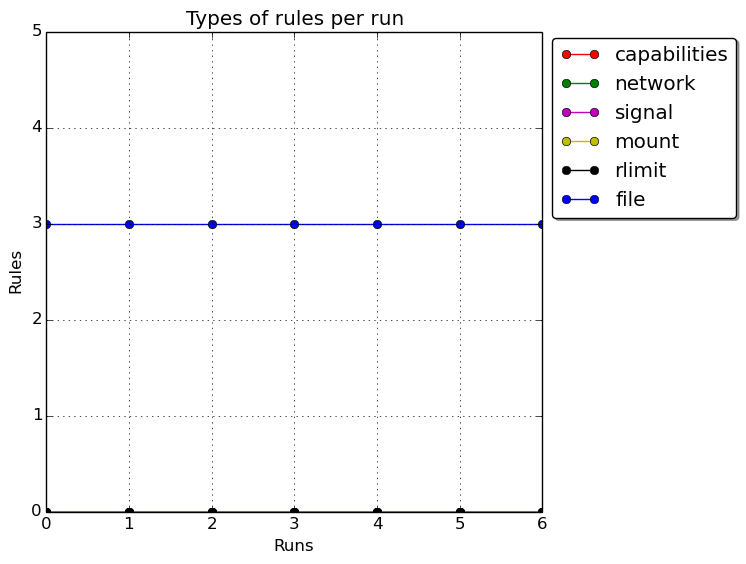
\includegraphics[width=0.64\linewidth]{./figures/mediastreaming/plots_with_grid/types_cloudsuitemedia-streamingdataset.png}
   \caption{Dataset's types of rules per run}
\end{figure}
